%% Chapter 6 — Component Selection & Datasheet Literacy
%% Course 247-519-VA, Vanier College
%% Project Planning & Prototyping

\chapter{Component Selection \& Datasheet Literacy}
\label{ch6}

\paragraph{Where this fits.}
You are now inside Stage~3 (Development), moving toward Gate~3.
Chapter~5 delivered the system block diagram and interface table --- the verified architecture with its contracts and budgets.
That gave you blocks to fill --- but not yet a method for choosing the components that will populate them.
This chapter teaches that method.
Component selection at Stage~3 locks in a large fraction of unit cost, reliability, and supply-chain risk before a single board is laid out; a poor choice here is expensive to reverse.
The deliverable you will carry into Gate~3 is a \textbf{component selection table}\index{component selection table} for the critical path of your prototype: part number, supplier, lifecycle status, derating factor, operating margin, alternate part, and system MTBF.

By the end of this chapter you will be able to:
\begin{enumerate}
  \item extract the four critical parameter zones from a component datasheet (absolute maximum ratings, recommended operating conditions, electrical characteristics, timing diagrams);
  \item apply derating factors to select components with adequate operating margin;
  \item evaluate a component's lifecycle status using manufacturer product-page data;
  \item identify a viable second source that satisfies parametric equivalence, footprint compatibility, and Active lifecycle status; and
  \item estimate the failure rate of a series system from individual component MTBF values.
\end{enumerate}

% ─────────────────────────────────────────────────────────────────────────────
\section{Reading a Datasheet}
\label{sec:ch6-datasheet}
% ─────────────────────────────────────────────────────────────────────────────

A \textbf{datasheet}\index{datasheet} is the manufacturer's binding specification for a component.
It is not a tutorial, a marketing document, or a suggestion.
Every number in a datasheet has a precise meaning, and your ability to extract and apply those numbers correctly separates a reliable design from one that fails unpredictably in the field.

You read a datasheet in a fixed order.
You do not read from page one to the end.
They go directly to four zones --- in the order listed below --- before they read anything else.
Figure~\ref{fig:ch6-datasheet} annotates the anatomy of a representative datasheet, marking each of the four zones.

\begin{figure}[htbp]
  \centering
  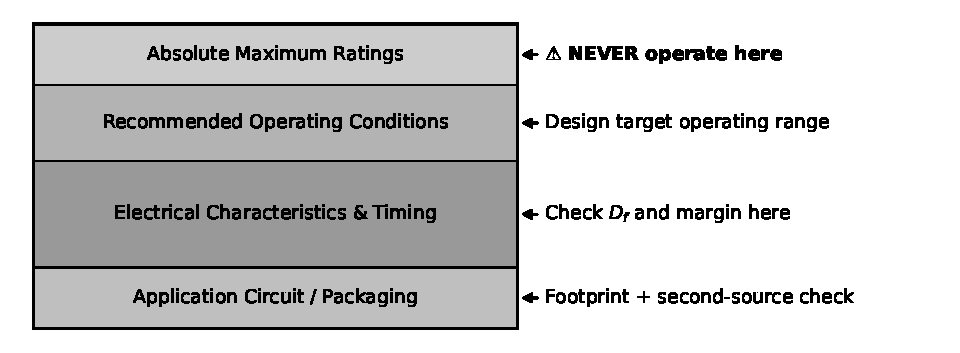
\includegraphics[width=0.90\textwidth]{images/fig_01_datasheet_anatomy}
  \caption{Annotated anatomy of a component datasheet showing the four critical
           zones: (1)~absolute maximum ratings, (2)~recommended operating
           conditions, (3)~electrical characteristics, and (4)~timing diagrams.
           Zone boundaries and key parameters are highlighted.
           Application circuit and packaging sections are labelled but not
           highlighted because they are consulted after the four critical zones
           are verified.}
  \label{fig:ch6-datasheet}
\end{figure}

\subsection{Zone 1 — Absolute Maximum Ratings}
\label{sec:ch6-abs-max}

\textbf{Absolute maximum ratings}\index{absolute maximum ratings} are the values beyond which permanent damage to the component is possible.
They are not operating limits.
The word ``maximum'' does not mean ``allowed operating point'' --- it means ``do not exceed under any condition, even briefly, or the silicon, ceramic, or polymer may be permanently damaged.''
A component operated at its absolute maximum voltage may work today, tomorrow, and for a week.
It may also degrade silently and fail during the customer demonstration.
The manufacturer guarantees \emph{nothing} about behaviour at or above these limits.

When you open a new datasheet, find the absolute maximum ratings table first.
Write down the supply voltage maximum, the maximum junction temperature, and the maximum input voltage at any pin you plan to drive.
These are your hard fences.

\subsection{Zone 2 — Recommended Operating Conditions}
\label{sec:ch6-rec-op}

\textbf{Recommended operating conditions}\index{recommended operating conditions} are the voltage, current, temperature, and frequency ranges within which the manufacturer tests the component and guarantees all published electrical characteristics.
These limits are significantly narrower than absolute maximum ratings.
Operating inside the recommended conditions is the minimum standard for a professional design.

The gap between the recommended operating limit and the absolute maximum limit is not a design margin you are allowed to use.
It is a zone the manufacturer reserves for statistical variation, lot-to-lot spread, and the mathematical uncertainty in their own test equipment.
You will learn in Section~\ref{sec:ch6-derating} that professional practice requires you to stay inside the recommended conditions, and then to derate further from there.

\subsection{Zone 3 — Electrical Characteristics}
\label{sec:ch6-elec-char}

\textbf{Electrical characteristics}\index{electrical characteristics} tables list the guaranteed minimum, typical, and maximum values for every important parameter: output voltage, quiescent current, input impedance, propagation delay, leakage current, and dozens more.
The columns are labelled Min, Typ, and Max.

This is the single most important discipline in datasheet reading: \textbf{design to the Min and Max columns, never to the Typ column.}
The typical value describes the median part from the manufacturer's characterisation lot.
Your prototype will contain parts from many lots, spanning a temperature range and an aging curve.
If your circuit only works when every component happens to hit its typical value, your circuit does not work --- it occasionally works.

\subsection{Zone 4 — Timing Diagrams}
\label{sec:ch6-timing}

\textbf{Timing diagrams}\index{timing diagram} specify the temporal relationships between signals: setup time, hold time, propagation delay, clock-to-output delay, and bus turn-around time.
These parameters are what make the interface contracts from Chapter~5 enforceable at the component level.

Recall from Chapter~5 that the running-example sorter has a fixed timing budget of 5~ms from sensor trigger to actuator command, with zero margin.
That zero-margin budget means that every component on the signal path must be verified against its timing parameters in Zone~4 before it is selected.
If a motor driver's datasheet shows a command-propagation delay of 2.1~ms worst-case, and you had allocated only 2~ms for that subsystem, the component violates the interface contract --- regardless of what the typical value says.

\subsection{Application Circuits and Packaging}
\label{sec:ch6-app-pkg}

After you have verified all four critical zones, two additional sections become relevant.
\textbf{Application circuits}\index{application circuit} show the manufacturer's recommended decoupling topology, external component values, and layout guidance.
Follow these circuits as a starting point; deviating from them requires justification.
The \textbf{packaging and footprint}\index{packaging} section specifies the physical dimensions and land pattern for PCB layout.
Mismatching a footprint to the physical component is one of the most common and most embarrassing prototype failures --- a component that cannot be soldered to the board it was designed for.

% ─────────────────────────────────────────────────────────────────────────────
\section{Derating}
\label{sec:ch6-derating}
% ─────────────────────────────────────────────────────────────────────────────

\textbf{Derating}\index{derating} is the practice of operating a component at a fraction of its rated limit in order to reduce the probability of failure and extend service life.
It is not a safety factor added out of conservatism --- it is a quantified, defensible engineering decision backed by decades of field-failure data.
The fundamental observation is that component failure rate increases nonlinearly as operating stress approaches the rated limit.
Figure~\ref{fig:ch6-derating} shows the characteristic stress--failure-rate curve: failure rate is roughly flat at low stress fractions, rises steeply as the fraction approaches 1.0, and becomes essentially unbounded above the absolute maximum.

\begin{figure}[htbp]
  \centering
  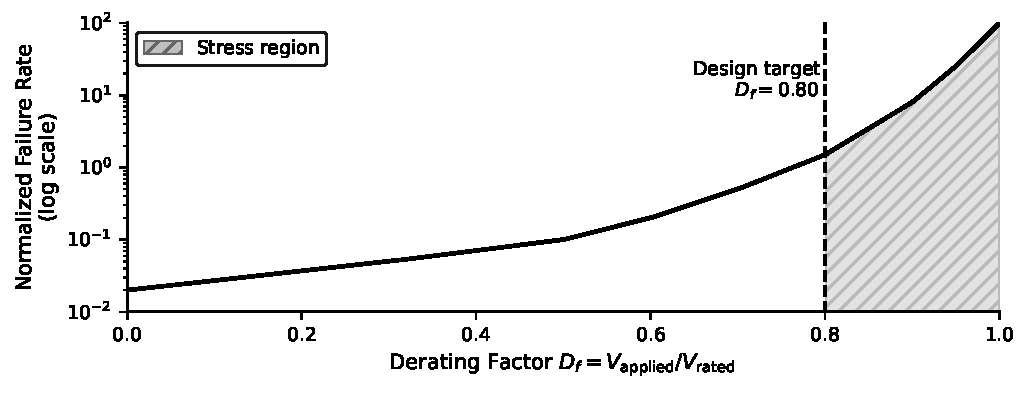
\includegraphics[width=0.85\textwidth]{images/fig_02_derating_curve}
  \caption{Component failure rate as a function of derating factor $D_f$.
           The curve is approximately flat below $D_f = 0.5$ and rises sharply
           above $D_f = 0.8$.
           The shaded region between $D_f = 0.8$ and $D_f = 1.0$ represents
           the stress zone where failure rate accelerates; the region above
           $D_f = 1.0$ (absolute maximum) represents the damage zone.
           The dashed line at $D_f = 0.80$ marks the maximum acceptable
           derating factor for voltage in this course.}
  \label{fig:ch6-derating}
\end{figure}

The \textbf{derating factor}\index{derating factor} for a given parameter is defined as:

\begin{equation}\label{eq:ch6-derating}
  D_f = \frac{V_{\text{applied}}}{V_{\text{rated}}}
\end{equation}

where $V_{\text{applied}}$ is the actual operating value and $V_{\text{rated}}$ is the component's rated limit for that parameter.
Although Equation~\ref{eq:ch6-derating} is written in terms of voltage, the same ratio applies to current, power dissipation, and any other stress parameter.

The derating targets used in this course are:

\begin{itemize}
  \item \textbf{Voltage (semiconductor):} $D_f \leq 0.80$
  \item \textbf{Voltage (capacitor):} $D_f \leq 0.75$
  \item \textbf{Current (semiconductor junction):} $D_f \leq 0.75$
  \item \textbf{Power dissipation:} $D_f \leq 0.70$
  \item \textbf{Junction temperature:} operate at least 25~°C below rated maximum junction temperature
\end{itemize}

These targets are conservative relative to some industry standards and are appropriate for a prototype context where accelerated testing and statistical sampling are not available.

\paragraph{Common Pitfalls.}
\begin{itemize}
  \item \textbf{Operating at absolute maximum ratings.}
        A component that operates at its absolute maximum voltage in a lab environment --- with stable bench power, 22~°C ambient, and no vibration --- will not reproduce that environment in a factory, a warehouse, or a field installation.
        ``It worked in the lab'' is not a reliability argument.
        The absolute maximum ratings exist to describe the damage threshold; the only correct interpretation is ``never go here.''
  \item \textbf{No second source identified at design time.}
        A component selected without an identified alternate forces a design respin if the primary supplier discontinues or allocates the part.
        The respin cost, measured in engineering hours and schedule delay, routinely exceeds the original prototype budget.
        See Section~\ref{sec:ch6-secondsource} for the formal second-sourcing process.
  \item \textbf{Accepting a component because a colleague used it before.}
        A colleague's previous use of a component tells you that it worked in one set of operating conditions, in one design, at one point in time.
        It does not tell you that the component is active in the supply chain today, that it meets your design's specific voltage and timing requirements, or that it is available in the quantity your production ramp requires.
        Always check lifecycle status and verify the new design's specific operating conditions against the datasheet, regardless of prior familiarity.
\end{itemize}

% ─────────────────────────────────────────────────────────────────────────────
\section{Operating Margin}
\label{sec:ch6-margin}
% ─────────────────────────────────────────────────────────────────────────────

Where derating describes how close you are operating to the component's stress limit, \textbf{operating margin}\index{operating margin} describes how much headroom remains between an actual measured value and a specification limit.
The two quantities are related but distinct.
Derating is a design decision you make before building; margin is a measurement you make after building or simulating, to verify that the design decision was sufficient.

Operating margin is defined as:

\begin{equation}\label{eq:ch6-margin}
  M = \frac{\text{spec limit} - \text{actual value}}{\text{spec limit}} \times 100\%
\end{equation}

A positive $M$ means the actual value is inside the specification --- you have headroom.
A negative $M$ means the actual value has violated the specification --- the design fails.
A margin of zero means the design is on the edge: any variation in temperature, supply voltage, component tolerance, or aging will push it into failure.

You should target a minimum margin of 20\% on timing parameters and 25\% on voltage parameters for a first prototype.
These targets give you room to absorb the variation you will discover when you measure actual hardware for the first time.

% ─────────────────────────────────────────────────────────────────────────────
\section{Component Lifecycle Status}
\label{sec:ch6-lifecycle}
% ─────────────────────────────────────────────────────────────────────────────

Every active component has a \textbf{lifecycle status}\index{lifecycle status} that describes where it sits in the manufacturer's product line plan.
Treat lifecycle status as a risk register entry, not a purchasing footnote.
Selecting a component without verifying its lifecycle status is equivalent to building a feature on a third-party API without checking its deprecation schedule.

Figure~\ref{fig:ch6-lifecycle} shows the standard lifecycle timeline with risk annotations for each phase.

\begin{figure}[htbp]
  \centering
  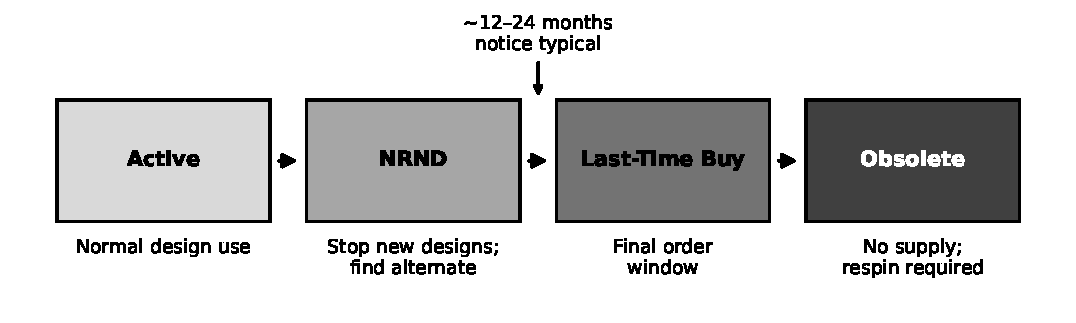
\includegraphics[width=0.92\textwidth]{images/fig_03_lifecycle}
  \caption{Component lifecycle timeline.
           Phases from left to right: Introduction, Growth, Mature (Active),
           NRND, Last-Time Buy, and Obsolete.
           Risk annotations indicate the design action appropriate at each
           phase.
           The bracket labelled ``Design Window'' spans Introduction through
           Mature; the bracket labelled ``Risk Window'' spans NRND through
           Last-Time Buy.}
  \label{fig:ch6-lifecycle}
\end{figure}

The four statuses you will encounter on distributor websites and manufacturer product pages are:

\begin{itemize}
  \item \textbf{Active}\index{lifecycle status!active}: The component is in full production.
        The manufacturer is actively taking orders, maintaining inventory, and providing technical support.
        This is the only lifecycle status that is acceptable for a new design without a written risk exception.

  \item \textbf{NRND (Not Recommended for New Designs)}\index{NRND}\index{lifecycle status!NRND}: The manufacturer is signalling that the component is approaching end-of-life.
        NRND does not mean ``unavailable today'' --- it means ``do not start a new design on this component.''
        The typical window between NRND announcement and end-of-life is 12--36 months, but this varies widely.
        If a component you are considering is in NRND status, you must find an alternative before design freeze.
        Specifically, two actions are required: (1)~identify an Active-status replacement that meets all parametric and footprint criteria; and (2)~record the NRND status as a risk register entry with a resolution deadline.

  \item \textbf{Last-Time Buy (LTB)}\index{lifecycle status!last-time buy}: The manufacturer has announced a final production run.
        Orders must be placed by a specified date.
        After that date the component will never be manufactured again.
        An LTB component should never be selected for a new design unless a complete lifetime supply can be purchased, inspected, and stored --- a practice reserved for high-reliability aerospace and medical applications, not prototypes.

  \item \textbf{Obsolete}\index{lifecycle status!obsolete}: The component is no longer available from the manufacturer.
        It may still appear on the secondary market (broker stock), but secondary-market parts carry risks of counterfeiting, improper storage, and undocumented handling that are unacceptable for a professional design.
\end{itemize}

\paragraph{In Practice.}
A team at a previous cohort built a working prototype on an MCU that was listed as Active at the time of component selection.
Six months after design freeze --- before the first production run --- the manufacturer moved that MCU to NRND status.
The team did not have a second source identified, because second-sourcing had been deferred.
The redesign to a compatible MCU required new firmware validation, a new schematic review, and a new round of regulatory EMC testing.
The total cost of the redesign exceeded the original prototype budget.
Lifecycle status must be verified at component selection, not at production planning.

% ─────────────────────────────────────────────────────────────────────────────
\section{Second-Sourcing Strategy}
\label{sec:ch6-secondsource}
% ─────────────────────────────────────────────────────────────────────────────

Once you have confirmed Active status for every critical-path component, the next obligation is to ensure you are not dependent on a single supplier.

A \textbf{second source}\index{second source} is an alternative component that can substitute for the primary selection without requiring a schematic change, a firmware change, or a re-qualification test.
Identifying a second source at component selection time costs roughly two hours of engineering effort.
Scrambling to find one after a supply disruption costs weeks.

A viable second source must satisfy three criteria simultaneously.
Satisfying two out of three is not sufficient:

\begin{enumerate}
  \item \textbf{Parametric equivalence}\index{parametric equivalence}: The alternate component must meet or exceed every specification that your design depends on --- not just the headline spec, but every parameter you extracted from Zones~1 through~4.
        A motor driver with the same current rating but a slower PWM frequency response is not parametrically equivalent if your control loop depends on the frequency response.

  \item \textbf{Footprint compatibility}\index{footprint compatibility}: The alternate component must be pin-compatible with the primary on the PCB land pattern.
        A component with identical electrical specifications but a different package (e.g., QFN-32 versus TQFP-32) requires a layout change, which in a professional context triggers a new design revision and new board fabrication.
        For a prototype, this is a measurable cost.

  \item \textbf{Lifecycle status}\index{lifecycle status}: The alternate component must itself be in Active status.
        An alternate that is NRND or LTB provides no protection against the supply disruption you are trying to mitigate.
\end{enumerate}

\paragraph{In Practice.}
A team locked their BOM fourteen weeks before the scheduled system integration test.
Three weeks later, the primary MCU lead time extended from stock to 14 weeks due to an industry allocation event.
Because the team had not identified a second source, they were unable to substitute an equivalent part.
The project schedule slipped by one full milestone --- losing a Stage-Gate review cycle --- while the team waited for allocation to clear.
Had a second source been identified at BOM lock, the swap could have been made within two days.

% ─────────────────────────────────────────────────────────────────────────────
\section{Supply Chain Risk}
\label{sec:ch6-supply}
% ─────────────────────────────────────────────────────────────────────────────

Component selection is not complete until you have assessed the supply chain risk of every part on the critical path.
\textbf{Supply chain risk}\index{supply chain risk} encompasses three main categories.

\textbf{Single-source components}\index{single-source component} are manufactured by exactly one supplier with no compatible alternate.
They represent the highest supply chain risk in a BOM.
When you identify a single-source component, it becomes a risk register entry (see Chapter~4) with a severity proportional to how difficult it would be to re-architect the design around a different part.

\textbf{Lead time}\index{lead time} is the calendar time between placing an order and receiving parts.
For most standard components, lead time is one to five weeks from distributor stock.
For certain microcontrollers, power management ICs, and RF transceivers, lead time from the factory can reach 26--52 weeks during periods of high demand.
You must verify the lead time of every critical-path component at the time of BOM lock, not at the time of purchase order.
Lead times reported on distributor websites are real-time and can change daily.

\textbf{Allocation periods}\index{allocation period} occur when a component is in higher demand than the manufacturer's capacity can supply.
During allocation, distributors receive fractional fills on their purchase orders, and small customers (including most prototype projects) may receive nothing.
Allocation periods for popular MCU families have historically lasted 12--24 months.
The only reliable mitigation is to have a qualified second source with independent supply chain.

% ─────────────────────────────────────────────────────────────────────────────
\section{MTBF and Reliability Basics}
\label{sec:ch6-mtbf}
% ─────────────────────────────────────────────────────────────────────────────

\textbf{Reliability}\index{reliability} is the probability that a system performs its required function for a specified time under specified conditions.
Every component you add to a system adds a probability of failure.
Understanding how to estimate the aggregate reliability of a multi-component path allows you to make informed decisions about which components to derate more aggressively, which to make redundant, and which to flag as reliability risks in the Gate~3 review.

\subsection{Failure Rate and FIT}
\label{sec:ch6-fit}

Component reliability is quantified by the \textbf{failure rate}\index{failure rate} $\lambda$, defined as the expected number of failures per unit time.
The industry-standard unit is the \textbf{FIT}\index{FIT} (Failures In Time), where:
\[
  1~\mathrm{FIT} = 1~\text{failure per}~10^{9}~\text{hours}
\]
A component with $\lambda = 200~\mathrm{FIT}$ is expected to produce one failure in $5 \times 10^6$ hours of aggregate device operation.
FIT values are published by manufacturers in reliability reports and can also be estimated using MIL-HDBK-217 or Telcordia SR-332 models, which account for operating temperature and applied stress.

\subsection{Series System Reliability}
\label{sec:ch6-series}

In a series reliability model, every component must function for the system to function.
This is the correct model for a critical signal path: if any component in the path fails, the path fails.
For a series system of $n$ components, the system failure rate and system MTBF are:

\begin{equation}\label{eq:ch6-lambda-sys}
  \lambda_{\text{sys}} = \sum_i \lambda_i, \qquad \mathrm{MTBF}_{\text{sys}} = \frac{1}{\lambda_{\text{sys}}}
\end{equation}

where $\lambda_i$ is the failure rate of the $i$-th component and all rates are in consistent units (FITs or failures per hour).
Note that adding components to a series path always \emph{decreases} system MTBF.
This is the quantitative justification for minimising component count on reliability-critical paths.

\subsection{Parallel Redundancy}
\label{sec:ch6-parallel}

When two or more components perform the same function in parallel --- and the system succeeds if at least one survives --- the reliability model changes.
For a parallel set of $n$ components each with reliability $R_i$, the system reliability is:

\begin{equation}\label{eq:ch6-parallel}
  R_{\text{sys}} = 1 - \prod_i (1 - R_i)
\end{equation}

where $R_i$ is the probability that component $i$ has not failed over the mission time.
Parallel redundancy is used in safety-critical subsystems --- power supplies, communication links, and actuator drivers where a single failure must not halt the system.
It is not a substitute for derating; a redundant pair of poorly derated components has a higher aggregate failure rate than a single well-derated component.

% ─────────────────────────────────────────────────────────────────────────────
\section{Worked Example}
\label{sec:ch6-worked}
% ─────────────────────────────────────────────────────────────────────────────

\subsection{Part A — Derating and Operating Margin for an MCU}
\label{sec:ch6-worked-a}

The running-example sorter uses an STM32-class MCU with the following datasheet parameters:
\begin{itemize}
  \item Rated supply voltage: $V_{\text{rated}} = 3.6~\mathrm{V}$
  \item Applied supply voltage: $V_{\text{applied}} = 3.3~\mathrm{V}$
  \item Ambient temperature: $T_{\text{ambient}} = 85~\mathrm{°C}$
  \item Timing parameter spec limit (setup time): $t_{\text{spec}} = 10~\mathrm{ns}$
  \item Timing parameter measured actual value: $t_{\text{actual}} = 3.2~\mathrm{ns}$
\end{itemize}

\textbf{Derating factor for supply voltage} (Equation~\ref{eq:ch6-derating}):
\[
  D_f = \frac{V_{\text{applied}}}{V_{\text{rated}}} = \frac{3.3~\mathrm{V}}{3.6~\mathrm{V}} = 0.917
\]

Comparing to the derating target of $D_f \leq 0.80$ stated in Section~\ref{sec:ch6-derating}: $D_f = 0.917$ \textbf{exceeds the target}.
The MCU supply voltage does not comply with the course derating rule.
This finding must be recorded as a risk item.

\paragraph{Design action required.}
$D_f = 0.917 > 0.80$ fails the course derating target.
This entry \textbf{must be flagged} in the component selection table and must be resolved --- by selecting a component with $V_{\text{rated}} \geq 4.1$~V or by lowering $V_{\text{applied}}$ to comply --- before Gate~3 will accept the deliverable.

The design team must either reduce $V_{\text{applied}}$ (for example, reducing $V_{\text{applied}}$ to 2.88~V gives $D_f = 2.88/3.6 = 0.80$ (the boundary), or to 2.7~V gives $D_f = 2.7/3.6 = 0.75$ (compliant)) or select a component with a higher rated supply voltage.

\textbf{Operating margin on the timing parameter} (Equation~\ref{eq:ch6-margin}):
\[
  M = \frac{10~\mathrm{ns} - 3.2~\mathrm{ns}}{10~\mathrm{ns}} \times 100\% = \frac{6.8~\mathrm{ns}}{10~\mathrm{ns}} \times 100\% = 68\%
\]

A margin of 68\% on the setup time is well above the 20\% target for timing parameters.
The setup time is not the constraint on this design.
However, note that the 5~ms end-to-end timing budget from Chapter~5 has zero margin at the system level; the comfortable margin on this individual timing parameter does not relieve the pressure on the full pipeline.

\subsection{Part B — System MTBF for the Actuator Interface Path}
\label{sec:ch6-worked-b}

The actuator interface path in the running-example sorter consists of three components in series: the MCU, a level-shifter, and a motor driver.
Their failure rates are:

\begin{center}
\begin{tabular}{llr}
  \hline
  Component & Role & $\lambda$ (FIT) \\
  \hline
  MCU (STM32-class) & Firmware execution, actuator command & 200 \\
  Level-shifter & 3.3~V to 5~V translation & 50 \\
  Motor driver & Sort actuator PWM control & 400 \\
  \hline
\end{tabular}
\end{center}

\textbf{System failure rate} (Equation~\ref{eq:ch6-lambda-sys}):
\[
  \lambda_{\text{sys}} = 200 + 50 + 400 = 650~\mathrm{FIT}
\]

\textbf{System MTBF in hours}:
\[
  \mathrm{MTBF}_{\text{sys}} = \frac{1}{\lambda_{\text{sys}}} = \frac{10^{9}~\mathrm{hours}}{650} \approx 1{,}538{,}462~\mathrm{hours}
\]

\textbf{Expressing MTBF in years} (dividing by 8760 hours per year):
\[
  \mathrm{MTBF}_{\text{sys}} = \frac{1{,}538{,}462}{8{,}760} \approx 175.6~\mathrm{years}
\]

The motor driver dominates the system failure rate with 62\% of the total $\lambda_{\text{sys}}$.
If the project reliability target requires a higher MTBF, the motor driver is the first component to investigate for a lower-FIT alternative.
The level-shifter contributes only 8\% of total failure rate and is not the priority for improvement.

% ─────────────────────────────────────────────────────────────────────────────
\section{Try It Yourself}
\label{sec:ch6-tiy}
% ─────────────────────────────────────────────────────────────────────────────

The following problem uses different numbers from the worked example.
Work through each part before consulting the solutions in the appendix.

A 5~V linear regulator has the following datasheet and measurement data:
\begin{itemize}
  \item Rated supply voltage: $V_{\text{rated}} = 5.5~\mathrm{V}$
  \item Applied supply voltage: $V_{\text{applied}} = 4.8~\mathrm{V}$
  \item Timing parameter spec limit (output-settle time): $t_{\text{spec}} = 20~\mathrm{\mu s}$
  \item Timing parameter measured actual value: $t_{\text{actual}} = 14~\mathrm{\mu s}$
\end{itemize}

Two components on the sensor front-end critical path:
\begin{itemize}
  \item Sensor: $\lambda_1 = 120~\mathrm{FIT}$
  \item Analog front-end IC: $\lambda_2 = 310~\mathrm{FIT}$
\end{itemize}

\begin{enumerate}
  \item[(a)] Compute $D_f$ for the supply voltage using Equation~\ref{eq:ch6-derating}.
             Is the result within the $D_f \leq 0.80$ voltage derating target?

  \item[(b)] Compute the operating margin $M$ on the timing parameter using
             Equation~\ref{eq:ch6-margin}.

  \item[(c)] Compute $\lambda_{\text{sys}}$ and $\mathrm{MTBF}_{\text{sys}}$ for the two-component
             series path using Equation~\ref{eq:ch6-lambda-sys}.
             Express MTBF in years (divide hours by 8{,}760).

  \item[(d)] The sensor is currently listed as NRND by its manufacturer.
             State the two actions defined in Section~\ref{sec:ch6-lifecycle} that the team must complete before the next design review, and give the lifecycle status the replacement component must hold.
\end{enumerate}

% ─────────────────────────────────────────────────────────────────────────────
\section{Review Questions}
\label{sec:ch6-review}
% ─────────────────────────────────────────────────────────────────────────────

\begin{enumerate}
  \item[\textbf{Q1.}] Explain the difference between ``absolute maximum ratings'' and ``recommended operating conditions'' in a datasheet.
        Why is operating at the absolute maximum ratings a professional mistake, even if the component does not fail immediately?

  \item[\textbf{Q2.}] A component's lifecycle status changes from ``Active'' to ``NRND.''
        State what NRND means, the typical time window before end-of-life, and the two responses a design team should take within that window.

  \item[\textbf{Q3.}] A capacitor is rated at $V_{\text{rated}} = 16~\mathrm{V}$.
        The circuit applies $V_{\text{applied}} = 10~\mathrm{V}$.
        \begin{enumerate}
          \item[(a)] Compute $D_f$ using Equation~\ref{eq:ch6-derating}.
          \item[(b)] The derating rule for capacitors is $D_f \leq 0.75$.
                     Does this selection comply?
          \item[(c)] If $V_{\text{applied}}$ rises to 13~V under transient conditions,
                     recompute $D_f$ and state whether the component should be replaced.
        \end{enumerate}

  \item[\textbf{Q4.}] A four-component power path has failure rates
        $\lambda_1 = 80~\mathrm{FIT}$, $\lambda_2 = 150~\mathrm{FIT}$,
        $\lambda_3 = 220~\mathrm{FIT}$, $\lambda_4 = 90~\mathrm{FIT}$.
        \begin{enumerate}
          \item[(a)] Compute $\lambda_{\text{sys}}$ using Equation~\ref{eq:ch6-lambda-sys}.
          \item[(b)] Compute $\mathrm{MTBF}_{\text{sys}}$ in hours.
          \item[(c)] Convert to years (8{,}760 hours per year). Round to one decimal place.
          \item[(d)] The team adds a redundant parallel path for component~3 with an identical $\lambda_3 = 220$~FIT.
                     Using Equation~\ref{eq:ch6-parallel}, compute $R_{\text{sys}}$ for that redundant pair over a 10{,}000-hour mission time, where $R_i = e^{-\lambda_i t}$ with $\lambda_i$ in failures per hour (note: $1~\text{FIT} = 10^{-9}~\text{failures/hour}$).
                     State in one sentence whether the parallel pair improves or degrades reliability compared with a single component over the same mission time.
        \end{enumerate}

  \item[\textbf{Q5.}] Explain why a ``second source'' must satisfy three criteria ---
        parametric equivalence, footprint compatibility, and lifecycle status ---
        and give an example of a second source that satisfies two of the three
        but fails on one.
\end{enumerate}

% ─────────────────────────────────────────────────────────────────────────────
\section{End-of-Chapter Artifact}
\label{sec:ch6-artifact}
% ─────────────────────────────────────────────────────────────────────────────

The deliverable for this chapter is the \textbf{component selection table}\index{component selection table} for the critical path of your prototype.
This table is a mandatory input to Gate~3.
Complete one row per critical-path component using the template below.

\begin{center}
\small
\begin{tabular}{p{2.0cm}p{2.2cm}p{1.5cm}p{1.1cm}p{1.5cm}p{2.2cm}p{1.8cm}}
  \hline
  \textbf{Part number} &
  \textbf{Supplier} &
  \textbf{Lifecycle status} &
  \textbf{Derating factor $D_f$ (V)} &
  \textbf{Margin $M$ (\%)} &
  \textbf{Alternate part number} &
  \textbf{$\mathrm{MTBF}_{\text{sys}}$ (years)} \\
  \hline
  & & & & & & \\
  & & & & & & \\
  & & & & & & \\
  \hline
\end{tabular}
\end{center}

Column definitions:
\begin{itemize}
  \item \textbf{Lifecycle status}: Active, NRND, LTB, or Obsolete --- verified on the manufacturer's product page on the day of submission.
  \item \textbf{$D_f$ (V)}: Voltage derating factor computed using Equation~\ref{eq:ch6-derating}. Flag any value $> 0.80$ in red.
  \item \textbf{Margin $M$ (\%)}: Operating margin on the tightest timing or voltage parameter in the design, computed using Equation~\ref{eq:ch6-margin}. Flag any value $< 20\%$ in red.
  \item \textbf{Alternate part number}: A second source that satisfies all three criteria from Section~\ref{sec:ch6-secondsource}.
  \item \textbf{$\mathrm{MTBF}_{\text{sys}}$ (years)}: Computed using Equation~\ref{eq:ch6-lambda-sys} for the full critical path.
\end{itemize}

% ─────────────────────────────────────────────────────────────────────────────
\section{Summary}
\label{sec:ch6-summary}
% ─────────────────────────────────────────────────────────────────────────────

This chapter gave you the tools to fill the architecture blocks from Chapter~5 with verified components.
You can now navigate a datasheet systematically, extracting the four critical zones rather than reading from cover to cover.
You can apply derating factors and compute operating margins to quantify the headroom between your design's operating point and the component's limits.
You can assess lifecycle status and supply chain risk as engineering variables rather than purchasing footnotes, and identify a second source that genuinely substitutes for --- not just superficially resembles --- the primary selection.
Finally, you can estimate the MTBF of a series reliability path and use that estimate to identify which component on the critical path deserves the most engineering attention.

These competencies together constitute \textbf{datasheet literacy}\index{datasheet literacy}: the ability to translate a manufacturer's specification document into a set of verified, margin-positive design decisions.
A design built on verified components with documented margins and identified alternates is a design that can survive the surprises --- supply disruptions, temperature extremes, component lot variation --- that the prototype bench cannot anticipate.

Chapter~6 produced the component selection table --- part numbers, derating factors, lifecycle status, alternates, and system MTBF --- that locks the critical path into Gate~3.
Chapter~7 takes that table and examines how to design the assembly around those verified components so that manufacturing, testing, and serviceability are built in from the start.
